\chapter{数値実験}
\label{chap:experiment}

本章では,提案したアルゴリズムの有効性を検証するための実験を行う.
実験で比較するアルゴリズムは次の通り.
\begin{enumerate}
\item 再計算(Brandesのアルゴリズム)
  \par 辺が挿入または削除される度にBrandesのアルゴリズム(アルゴリズム\ref{algo:brandes})で媒介中心性を再計算する
\item 更新(提案手法)
  \par 辺が挿入または削除される度にアルゴリズム\ref{alg:proposed-algorithm-full}によって媒介中心性を更新する
\end{enumerate}

まず,人工ネットワークに対する実験を行う.ここでは,Brandesのアルゴリズムとの
比較や,更新したペア依存度の数と実行時間の関係,媒介中心性を更新した頂点数と
実際に媒介中心性が変化した頂点の関係を明らかにし,
第\ref{chap:complexity-analysis}章で行った理論的な解析結果との関連を示す.

次に,実ネットワークに対する実験を行う.この実験では,実ネットワークでの性能の比較および,
頑健な道路ネットワークの構築と,媒介中心性のリアルタイム計算への応用を想定した実験を行う.

なお,すべての実験は Intel (R) Xeon (R) CPU E-2620 v4 , 64GB RAM 上で行われた.
実験に用いたプログラムは gcc 7.2.0 によって, -O3 最適化フラグを付与してコンパイルされた.
プログラムのソースコードは\verb|github.com/y-satotani/dynamic-betweenness|で入手できる.

本節では,以下の項目について実験を行い,その結果について考察する.
\begin{enumerate}
\item Brandesのアルゴリズムとの比較
\item ペア依存度を更新した頂点ペアの数と実行時間の関係
\item 媒介中心性が実際に変化した頂点の数と更新した頂点の数の関係
\end{enumerate}

この実験では,次の二種類の人工ネットワークを対象とする.
\begin{enumerate}
\item Erd\H{o}s--R\'{e}nyiモデル\cite{Erdos1959}
\item Barab\'{a}si--Albertモデル\cite{Barabasi1999}
\end{enumerate}

\section{人工ネットワークに対する性能比較}

図\ref{fig:exp-artificial-order}は各アルゴリズムの実行時間を比較したものである.
各ネットワークの平均次数はおよそ$4$である.それぞれの頂点数について,
100個のネットワークに対する実行時間の最大値および平均値を計算している.

\begin{figure}[tb]
  \centering
  \includegraphics{exp-artificial-order.pdf}
  \caption{頂点数に対する実行時間の比較}
  \label{fig:exp-artificial-order}
\end{figure}

図\ref{fig:exp-artificial-order}より,二種類のネットワーク全てに対して,
頂点数が増加するとともに更新の平均実行時間が再計算のものと比べて短くなっていることが分かる.
ペア依存度を再計算する必要がある頂点が頂点数の増加とともに比較的少なくなることが理由と考えられる.

\input{exp-artificial.tex}

\section{実ネットワークに対する性能比較}

本節では,実ネットワークに対する実験を行う.
SNAPデータセット\cite{Leskovec2016}から取得した実ネットワークでの性能評価および,
頑健な道路ネットワークの構築と,媒介中心性のリアルタイム計算への応用を想定した実験を行う.

SNAPデータセットのいくつかの実ネットワークに対して,
提案手法とBrandesのアルゴリズムの比較実験を行った.
両アルゴリズムを各ネットワークに対して10回実行し,その実行時間の平均値および最大値を求めた.
実験結果を表\ref{tab:exp-real}に示す.

\input{exp-real.tex}

表\ref{tab:exp-real}より,提案手法は実ネットワークでも効率よく計算できることが確認できる.

\section{導出した計算量の妥当性の検証}

提案したアルゴリズムのようなオンラインアルゴリズムの性能を評価するためには,
アルゴリズムによって更新した要素の数を考慮する必要がある.
\cite{Ramalingam1996,Lee2012,Pontecorvi2014}
ここでは,ペア依存度を更新した頂点ペア数と実行時間の関係を実験によって
明らかにする.さらに,
第\ref{chap:complexity-analysis}章で行った理論的な解析結果と,
実際の計算時間の挙動に解離がないかを検証する.

図\ref{fig:exp-artificial-path-update}および図\ref{fig:exp-artificial-betw-update}はペア依存度を更新した頂点ペア数と実行時間の関係を表す.
頂点数を$1000$,平均次数は$4$または$64$とし,$100$個のネットワークに対してそれぞれ$1$回の更新を行った.

\begin{figure}[tb]
  \centering
  \includegraphics{exp-artificial-path-update.pdf}
  \caption{更新した頂点ペアの数に対する実行時間}
  \label{fig:exp-artificial-path-update}
\end{figure}

\begin{figure}[tb]
  \centering
  \includegraphics{exp-artificial-betw-update.pdf}
  \caption{更新した頂点ペアの数に対する実行時間}
  \label{fig:exp-artificial-betw-update}
\end{figure}

図\ref{fig:exp-artificial-path-update}および図\ref{fig:exp-artificial-betw-update}より,更新した頂点ペア数が少ないと,実行時間が短くなることが分かる.
さらに,次数が大きいと実行時間が長くなる.この性質は辺の数が増加すると実行時間も
増加することを示し,理論的な解析結果と一致する.

\section{冗長な走査の計数}

\textcolor{red}{書きかけ注意}
\begin{example}
  図\ref{fig:redundant-traverse}において$\delta_s(v_1)=\delta'_s(v_1)$であるが,
  $\delta_s(w_1)\neq\delta'_s(w_1)$である.
  同様に,$\delta_s(v_2)=\delta'_s(v_2)$であるが,$\sigma_{sv_2}\neq\sigma'_{sv_2}$である.
\end{example}

\begin{figure}[tb]
  \centering
  \def\svgwidth{.45\linewidth}
  \input{redundant-traverse.pdf_tex}
  \caption{冗長な走査の例}
  \label{fig:redundant-traverse}
\end{figure}

実際に媒介中心性が変化した頂点の数と$\lvert V_\delta\rvert$の関係について,一般的な議論は難しい.

\begin{example}
  図\ref{fig:redundant-traverse-many}のグラフにおいて,辺$\{V,W\}$を削除したときにアルゴリズムが
  ペア依存度を更新する頂点の数は$\lvert V_\delta\rvert\sim \lvert V\rvert$であるが,
  実際に媒介中心性が変化する頂点は$T,U,V,W$の$4$個である.

  \begin{figure}[tb]
    \centering
    \def\svgwidth{.8\linewidth}
    \input{redundant-traverse-many.pdf_tex}
    \caption{媒介中心性が変化しない頂点を多く更新する例}
    \label{fig:redundant-traverse-many}
  \end{figure}
\end{example}

第\ref{chap:complexity-analysis}章で行った理論解析では,
媒介中心性を更新した頂点の数と実際に媒介中心性が変化した頂点の数との
間の関係が不明なままであった.ここでは,その関係を実験的に明らかにする.

図\ref{fig:exp-artificial-phony}に,媒介中心性を更新した頂点の数と
実際に媒介中心性が変化した頂点の数の関係を示す.

\begin{figure}[tb]
  \centering
  \includegraphics{exp-artificial-phony.pdf}
  \caption{媒介中心性が変化した頂点数に対する,更新した頂点の数}
  \label{fig:exp-artificial-phony}
\end{figure}

\section{道路ネットワークを頑健にする辺操作}

第\ref{chap:introduction}章でも述べたように,道路ネットワークの頑健性を
向上するには,道路の建設によって媒介中心性の最大値を最小化する必要がある.
そこで,この実験では,実際の道路ネットワークに辺を挿入することによって,
媒介中心性の最大値を最小化させる.

道路ネットワークはOpenStreetMap\cite{OpenStreetMap}を利用して独自に構築した.
実験で用いる道路ネットワークを図\ref{fig:road-okayama}に示す.
このネットワークは$12165$個の頂点と$14820$本の辺を有する.

\begin{figure}[tb]
  \centering
  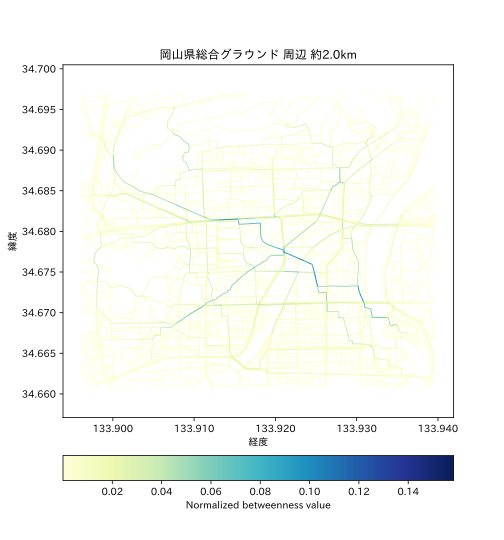
\includegraphics[width=.6\textwidth]{road-oka-with-betweenness.eps}
  \caption{実験で用いる道路ネットワーク}
  \label{fig:road-okayama}
\end{figure}

図\textcolor{red}{TODO}は辺操作後の媒介中心性の最大値の分布を表す.
辺の追加によって,最大$0.1607$の正規化された媒介中心性を
\textcolor{red}{xxx}まで減少させることに成功した.
また,辺の追加によって,最大$0.1607$の正規化された媒介中心性を
\textcolor{red}{xxx}まで減少させることに成功した.

\textcolor{red}{TODO: insert histogram of diff of min, mean, and max}

\textcolor{red}{TODO: insert figure of road indicates minimized maximum bc}

\section{媒介中心性のリアルタイム計算}

第\ref{chap:introduction}章で説明したように,社会ネットワーク分析に
おいて,媒介中心性をはじめとした中心性に注目することは重要である.
しかし,現実の社会ネットワークでは,友人関係が時間とともに出現と消滅を繰り返している.
この実験では,友人関係の出現と消滅が頻繁に起こりうる状況で,
媒介中心性をリアルタイムで計算する用途への応用を想定する.

この実験では,SFHH\cite{Genois2018}というデータセットを用いた.
このデータセットは,ある会議の参加者に赤外線タグを持たせることによって,
参加者同士の交流の様子を記録したものである.

図\ref{fig:exp-sfhh}は,そのSFHHデータセットをもとに,辺の挿入と削除を
繰り返したときの,各手法の実行時間を表す.それとともに,20秒間の
うちに発生した,挿入と削除操作の内訳を示す.

\begin{figure}[tb]
  \centering
  \includegraphics{exp-sfhh.eps}
  \caption{SFHHに対する実験結果}
  \label{fig:exp-sfhh}
\end{figure}

図より,小規模な場合ではあるが,媒介中心性をリアルタイムに計算できる.
しかし,更新の量が多い場合,Brandesのアルゴリズムの方が高速に計算していることが分かる.
今後は,多くの辺の操作に対応するアルゴリズムの開発が求められる.
